\documentclass[11pt,preprint, authoryear]{elsarticle}

\usepackage{lmodern}
%%%% My spacing
\usepackage{setspace}
\setstretch{1.2}
\DeclareMathSizes{12}{14}{10}{10}

% Wrap around which gives all figures included the [H] command, or places it "here". This can be tedious to code in Rmarkdown.
\usepackage{float}
\let\origfigure\figure
\let\endorigfigure\endfigure
\renewenvironment{figure}[1][2] {
    \expandafter\origfigure\expandafter[H]
} {
    \endorigfigure
}

\let\origtable\table
\let\endorigtable\endtable
\renewenvironment{table}[1][2] {
    \expandafter\origtable\expandafter[H]
} {
    \endorigtable
}


\usepackage{ifxetex,ifluatex}
\usepackage{fixltx2e} % provides \textsubscript
\ifnum 0\ifxetex 1\fi\ifluatex 1\fi=0 % if pdftex
  \usepackage[T1]{fontenc}
  \usepackage[utf8]{inputenc}
\else % if luatex or xelatex
  \ifxetex
    \usepackage{mathspec}
    \usepackage{xltxtra,xunicode}
  \else
    \usepackage{fontspec}
  \fi
  \defaultfontfeatures{Mapping=tex-text,Scale=MatchLowercase}
  \newcommand{\euro}{€}
\fi

\usepackage{amssymb, amsmath, amsthm, amsfonts}

\def\bibsection{\section*{References}} %%% Make "References" appear before bibliography


\usepackage[round]{natbib}

\usepackage{longtable}
\usepackage[margin=2.3cm,bottom=2cm,top=2.5cm, includefoot]{geometry}
\usepackage{fancyhdr}
\usepackage[bottom, hang, flushmargin]{footmisc}
\usepackage{graphicx}
\numberwithin{equation}{section}
\numberwithin{figure}{section}
\numberwithin{table}{section}
\setlength{\parindent}{0cm}
\setlength{\parskip}{1.3ex plus 0.5ex minus 0.3ex}
\usepackage{textcomp}
\renewcommand{\headrulewidth}{0pt}

\usepackage{array}
\newcolumntype{x}[1]{>{\centering\arraybackslash\hspace{0pt}}p{#1}}

%%%%  Remove the "preprint submitted to" part. Don't worry about this either, it just looks better without it:
\makeatletter
\def\ps@pprintTitle{%
  \let\@oddhead\@empty
  \let\@evenhead\@empty
  \let\@oddfoot\@empty
  \let\@evenfoot\@oddfoot
}
\makeatother

 \def\tightlist{} % This allows for subbullets!

\usepackage{hyperref}
\hypersetup{breaklinks=true,
            bookmarks=true,
            colorlinks=true,
            citecolor=blue,
            urlcolor=blue,
            linkcolor=blue,
            pdfborder={0 0 0}}


% The following packages allow huxtable to work:
\usepackage{siunitx}
\usepackage{multirow}
\usepackage{hhline}
\usepackage{calc}
\usepackage{tabularx}
\usepackage{booktabs}
\usepackage{caption}


\newenvironment{columns}[1][]{}{}

\newenvironment{column}[1]{\begin{minipage}{#1}\ignorespaces}{%
\end{minipage}
\ifhmode\unskip\fi
\aftergroup\useignorespacesandallpars}

\def\useignorespacesandallpars#1\ignorespaces\fi{%
#1\fi\ignorespacesandallpars}

\makeatletter
\def\ignorespacesandallpars{%
  \@ifnextchar\par
    {\expandafter\ignorespacesandallpars\@gobble}%
    {}%
}
\makeatother

\newlength{\cslhangindent}
\setlength{\cslhangindent}{1.5em}
\newenvironment{CSLReferences}%
  {\setlength{\parindent}{0pt}%
  \everypar{\setlength{\hangindent}{\cslhangindent}}\ignorespaces}%
  {\par}


\urlstyle{same}  % don't use monospace font for urls
\setlength{\parindent}{0pt}
\setlength{\parskip}{6pt plus 2pt minus 1pt}
\setlength{\emergencystretch}{3em}  % prevent overfull lines
\setcounter{secnumdepth}{5}

%%% Use protect on footnotes to avoid problems with footnotes in titles
\let\rmarkdownfootnote\footnote%
\def\footnote{\protect\rmarkdownfootnote}
\IfFileExists{upquote.sty}{\usepackage{upquote}}{}

%%% Include extra packages specified by user

%%% Hard setting column skips for reports - this ensures greater consistency and control over the length settings in the document.
%% page layout
%% paragraphs
\setlength{\baselineskip}{12pt plus 0pt minus 0pt}
\setlength{\parskip}{12pt plus 0pt minus 0pt}
\setlength{\parindent}{0pt plus 0pt minus 0pt}
%% floats
\setlength{\floatsep}{12pt plus 0 pt minus 0pt}
\setlength{\textfloatsep}{20pt plus 0pt minus 0pt}
\setlength{\intextsep}{14pt plus 0pt minus 0pt}
\setlength{\dbltextfloatsep}{20pt plus 0pt minus 0pt}
\setlength{\dblfloatsep}{14pt plus 0pt minus 0pt}
%% maths
\setlength{\abovedisplayskip}{12pt plus 0pt minus 0pt}
\setlength{\belowdisplayskip}{12pt plus 0pt minus 0pt}
%% lists
\setlength{\topsep}{10pt plus 0pt minus 0pt}
\setlength{\partopsep}{3pt plus 0pt minus 0pt}
\setlength{\itemsep}{5pt plus 0pt minus 0pt}
\setlength{\labelsep}{8mm plus 0mm minus 0mm}
\setlength{\parsep}{\the\parskip}
\setlength{\listparindent}{\the\parindent}
%% verbatim
\setlength{\fboxsep}{5pt plus 0pt minus 0pt}



\begin{document}



\begin{frontmatter}  %

\title{How do oil price changes impact economic variables in the period
1990 to 2017: A Replication of the Cologni \& Manera paper}

% Set to FALSE if wanting to remove title (for submission)




\author[Add1]{Harriet Catherine Laing}
\ead{21617023@sun.ac.za}





\address[Add1]{Stellenbosch University, Stellenbosch, South Africa}



\vspace{1cm}





\vspace{0.5cm}

\end{frontmatter}



%________________________
% Header and Footers
%%%%%%%%%%%%%%%%%%%%%%%%%%%%%%%%%
\pagestyle{fancy}
\chead{}
\rhead{}
\lfoot{}
\rfoot{\footnotesize Page \thepage}
\lhead{}
%\rfoot{\footnotesize Page \thepage } % "e.g. Page 2"
\cfoot{}

%\setlength\headheight{30pt}
%%%%%%%%%%%%%%%%%%%%%%%%%%%%%%%%%
%________________________

\headsep 35pt % So that header does not go over title




\hypertarget{introduction}{%
\section{\texorpdfstring{Introduction
\label{Introduction}}{Introduction }}\label{introduction}}

To replicate the study by Cologni \& Manera, the sam methodology and
structural cointegrated VAR model was used. This paper investigates
whether the findings from Cologni \& Manera hold after 2003 in the
United States, as the economic impact of a rise in oil prices during the
period 1990 to 2017 is analysed.

Did the response of central banks reduce the impact of a sudden oil
price shock?

This replication paper finds that\ldots is the optimal model for this
time period and \ldots{}

\hypertarget{background}{%
\section{Background}\label{background}}

Many economists regard increases in the oil price as a major cause of
asymmetries in the business cycle. This issue became especially
important to economists following the world oil market highs in the
early 2000s which could lead to economic slowdowns in developed
countries. The hypothesised asymmetric relationship between oil prices
and economic activity was first hypothesised after the oil price
collapse of 1986 which did not lead to an economic boom, which is what
theoretically should have been the case following the view that there
existed an inverse relationship between oil prices and the economy.

However, the channels through which an increase in the oil price impacts
economic variables remains unclear. There are many possible theoretical
explanations; some of which link to the effect of decreasing firms'
profits which may reduce capital spending and consumers' expectations
which causes them to consume more today, others link to the income
transfer between oil-importing countries and oil exporting countries
that shifts, and others link an increase in oil prices to the increases
in prices of related goods, thereby increasing inflation.

There is also, importantly, effects on economic variables that flow
indirectly from an increase in oil prices. Namely, that the monetary
authority responds to increase employment and ensure price stability
once an increase in oil prices threatens these two objectives. For
example, in the US, the Federal bank \ldots{} The role of monetary
policy may cause delayed impacts of an increase in oil prices on
economic variables.

Many studies have found a negative impact on aggregate economic activity
as a result of an increase in the oil price (Hamilton, 1983).

\hypertarget{replication-methodology-results}{%
\section{Replication methodology \&
results}\label{replication-methodology-results}}

\hypertarget{step-1-find-the-data}{%
\section{Step 1: Find the data}\label{step-1-find-the-data}}

As per the paper, the data was sourced where possible from the IMF.
However, for the interest rate and exchange rate we sourced the data
from Board of Governors of the Federal Reserve System and for inflation
from the US Bureau of Labor Statistics. First, we want to use US data
and see if we can replicate the results in the study. We need to convert
all the data into quarterly. The time period available to reproduce the
results of the paper was constrained by the availability of world oil
price data: could only find from 1990, therefore had to limit to 1990
onwards. Similarly, restricted time period due to the data availability
of money. In the paper they used predominantly seasonally-adjusted data
but due to constraints on availability of data, for this replication I
used a combination of seasonally-adjusted and not seasonally-adjusted.

Interest Rate= Federal Funds Effective Rate, percent, not seasonally
adjusted, monthly Source: Board of Governors of the Federal Reserve
System Exchange Rate= Millions of Dollars, Not Seasonally Adjusted,
quarterly, source: Board of Governors of the Federal Reserve System
(2021) Inflation = Index 1982-1984=100, Seasonally Adjusted, monthly,
source U.S. Bureau of Labor Statistics Real GDP = Domestic Currency,
Seasonally Adjusted, quarterly, source IMF Monetary Aggregate = Dollars,
Seasonally Adjusted, monthly source: IMF World Oil Price = U.S. Dollars
per Barrel, Not Seasonally Adjusted, monthly, IMF. Need to do until 2017
because of monetary aggregate data constraints

The methodology that I applied in order to replicate the study, was to
first transform all of the quarterly series in logarithms except for the
interest rate. As in the paper, we run Augmented Dickey Fuller tests on
all the time series variables. Findings at the 1\% confidence interval
were that are all variables were non-stationary and were integrated of
order 1, except for the monetary aggregate which was found to be
integrated of order 2. The lags were selected according to the AIC
criteria, as done in the paper. The results in this replication differed
only from the paper regarding the integration order of inflation, which
was found to be integrated of order 1 by Cologni \& Manera. This
difference from the paper dictated that only the monetary aggregate be
transformed by subtracting inflation to become the real monetary
aggregate (by taking the difference between the logarithm of monetary
aggregate and the logarithm of inflation), and the transformation for
inflation was not followed. This is because for finding cointegrating
relationships, the time series variables must be integrated of order 1.

Resultant time series variables were as follows:

\begin{center}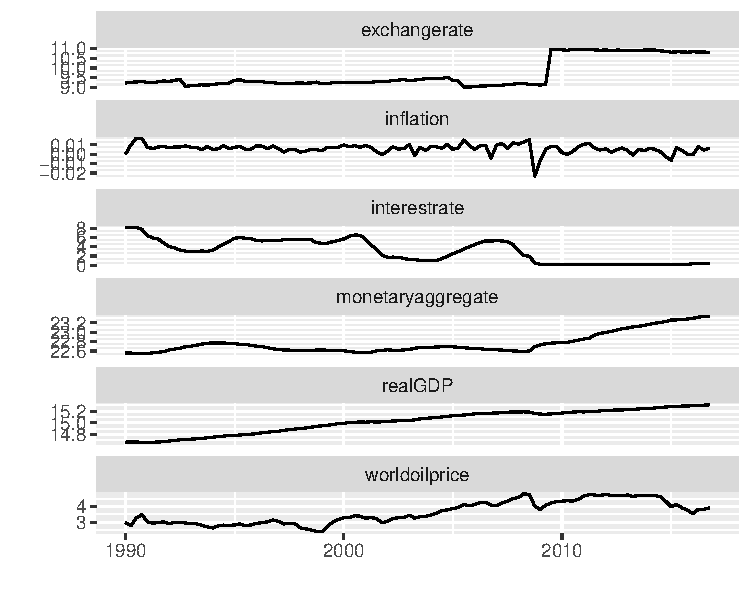
\includegraphics{README_files/figure-latex/unnamed-chunk-1-1} \end{center}

We then construct our VAR model by creating a matrix which includes the
time series variables included in Figure 1. We set the lag max to 4. The
VAR model was found to have 4 when we used the AIC lag selection
criteria and accounted for a time trend, as is done in the paper. We
order our VAR system in the same way as the short run restrictions
matrix in the paper: monetary aggregate, interest rate, real GDP,
inflation, exchange rate and world oil price. Lag should be 2 according
to the paper, but we find AIC suggests 4. As can be seen in Figure 1,
there is clearly a lot of persistence after the financial crisis.
Exchange rates for the US had a stark level increase around this
water-shed event and interest rates were set close to zero to try and
stimulate the economy, where they have remained fairly constant since
this monetary policy adjustment. Similarly, we can note real GDP has
diminished since 2008. Therefore, it is likely the difference in the
optimal lags between this replication and the Cologni \& Manera paper
arises from the different time periods used, as Cologni \& Manera's time
period ends before the financial crisis.

For a VAR model, we use the lag of 4, but for the VECM model we use the
lag of 3. This is because a VECM model has a difference term.

Now we can see long-run trends in the time series variables, but wish to
now see if there exists any cointegrating relationships. We test this
using the Johansen test, namely the eigenvalue test and the trace test.
For the eigenvalue test, we find that there is likely one cointegrating
relationship at the 5\% confidence interval where our critical value is
smaller than the test statistic, however, only marginally (37.26
estimated value \textless{} 37.52 critical value). For the trace test,
we find that there is at least two cointegrating relationships.
Therefore, because the rejection of the null hypothesis in the
eigenvalue test is incredibly marginal, we conclude from our estimates
that there is likely two cointegrating relationships. This is a
divergence from the result as is found for the US in Cologni \& Manera.

Cointegration analysis of the restricted system

We obtain the cointegrating vectors from the Johansen test and construct
a matrix is which each column is a cointegrating vector. Then we
multiply the VAR system by the cointegrating vector matrix to obtain the
error correction terms.

\begin{verbatim}
## #############
## ###Model VECM 
## #############
## Full sample size: 108    End sample size: 104
## Number of variables: 6   Number of estimated slope parameters 126
## AIC -3210.216    BIC -2855.868   SSR 74.89496
## Cointegrating vector (estimated by ML):
##    realGDP worldoilprice interestrate   inflation exchangerate
## r1       1             0   -0.1704922 -0.01710960    0.6161332
## r2       0             1    1.6056301  0.06991751   -5.4962156
##    monetaryaggregate
## r1        -0.3747751
## r2         6.5786487
## 
## 
##                            ECT1                ECT2               
## Equation realGDP           0.0114(0.0262)      0.0012(0.0029)     
## Equation worldoilprice     -1.1213(0.6892)     -0.1191(0.0757)    
## Equation interestrate      -0.8253(1.3364)     -0.0909(0.1468)    
## Equation inflation         1.9807(4.2269)      0.2323(0.4642)     
## Equation exchangerate      -1.5280(0.4970)**   -0.1498(0.0546)**  
## Equation monetaryaggregate -0.0999(0.0543).    -0.0127(0.0060)*   
##                            Intercept             realGDP -1          
## Equation realGDP           -0.2387(0.5689)       0.3017(0.1198)*     
## Equation worldoilprice     23.9522(14.9378)      6.0850(3.1445).     
## Equation interestrate      18.0500(28.9642)      9.3757(6.0972)      
## Equation inflation         -43.1723(91.6115)     23.9182(19.2849)    
## Equation exchangerate      31.3052(10.7722)**    0.0695(2.2676)      
## Equation monetaryaggregate 2.3668(1.1764)*       -0.2741(0.2476)     
##                            worldoilprice -1    interestrate -1    
## Equation realGDP           -0.0015(0.0061)     -0.0022(0.0021)    
## Equation worldoilprice     0.4921(0.1589)**    -0.0330(0.0553)    
## Equation interestrate      0.5017(0.3081)      0.5658(0.1072)***  
## Equation inflation         4.0209(0.9746)***   -0.8458(0.3391)*   
## Equation exchangerate      0.3216(0.1146)**    0.0338(0.0399)     
## Equation monetaryaggregate -0.0342(0.0125)**   0.0027(0.0044)     
##                            inflation -1        exchangerate -1    
## Equation realGDP           -0.0007(0.0010)     0.0030(0.0035)     
## Equation worldoilprice     -0.0649(0.0261)*    0.0232(0.0930)     
## Equation interestrate      -0.1333(0.0505)**   -0.0459(0.1802)    
## Equation inflation         -0.3031(0.1598).    0.2740(0.5701)     
## Equation exchangerate      -0.0376(0.0188)*    -0.2884(0.0670)*** 
## Equation monetaryaggregate 0.0093(0.0021)***   -0.0107(0.0073)    
##                            monetaryaggregate -1 realGDP -2           
## Equation realGDP           -0.0421(0.0628)      0.2444(0.1211)*      
## Equation worldoilprice     -0.5255(1.6486)      1.0297(3.1793)       
## Equation interestrate      -0.7766(3.1966)      -0.0562(6.1646)      
## Equation inflation         1.3461(10.1107)      -10.4541(19.4983)    
## Equation exchangerate      -0.3822(1.1889)      -5.2154(2.2927)*     
## Equation monetaryaggregate 0.3084(0.1298)*      -0.4686(0.2504).     
##                            worldoilprice -2    interestrate -2   
## Equation realGDP           0.0033(0.0061)      0.0020(0.0025)    
## Equation worldoilprice     0.0529(0.1609)      0.0008(0.0653)    
## Equation interestrate      -0.3103(0.3121)     0.0588(0.1266)    
## Equation inflation         0.8367(0.9870)      0.1164(0.4004)    
## Equation exchangerate      0.0028(0.1161)      0.0796(0.0471).   
## Equation monetaryaggregate -0.0030(0.0127)     0.0014(0.0051)    
##                            inflation -2        exchangerate -2    
## Equation realGDP           -0.0010(0.0010)     -0.0023(0.0034)    
## Equation worldoilprice     -0.0211(0.0266)     -0.0957(0.0890)    
## Equation interestrate      0.0222(0.0516)      -0.1919(0.1725)    
## Equation inflation         -0.1823(0.1633)     -0.6758(0.5456)    
## Equation exchangerate      -0.0071(0.0192)     -0.1283(0.0642)*   
## Equation monetaryaggregate 0.0023(0.0021)      -0.0097(0.0070)    
##                            monetaryaggregate -2 realGDP -3          
## Equation realGDP           0.0925(0.0628)       -0.0572(0.1260)     
## Equation worldoilprice     2.1871(1.6496)       -1.6558(3.3091)     
## Equation interestrate      4.6408(3.1985)       5.5340(6.4163)      
## Equation inflation         4.7544(10.1165)      -8.8125(20.2941)    
## Equation exchangerate      0.7138(1.1896)       -10.8377(2.3863)*** 
## Equation monetaryaggregate -0.0451(0.1299)      0.2839(0.2606)      
##                            worldoilprice -3   interestrate -3    
## Equation realGDP           0.0061(0.0059)     0.0007(0.0022)     
## Equation worldoilprice     0.2848(0.1541).    0.0895(0.0570)     
## Equation interestrate      1.2330(0.2988)***  0.0649(0.1105)     
## Equation inflation         0.4219(0.9450)     0.9330(0.3494)**   
## Equation exchangerate      0.3740(0.1111)**   -0.0451(0.0411)    
## Equation monetaryaggregate -0.0218(0.0121).   -0.0080(0.0045).   
##                            inflation -3        exchangerate -3    
## Equation realGDP           -0.0016(0.0010)     0.0017(0.0034)     
## Equation worldoilprice     -0.0329(0.0258)     -0.0271(0.0888)    
## Equation interestrate      -0.1358(0.0500)**   -0.0992(0.1721)    
## Equation inflation         -0.0726(0.1580)     -0.5133(0.5445)    
## Equation exchangerate      -0.1181(0.0186)***  -0.0048(0.0640)    
## Equation monetaryaggregate 0.0050(0.0020)*     -0.0079(0.0070)    
##                            monetaryaggregate -3
## Equation realGDP           -0.0568(0.0583)     
## Equation worldoilprice     -0.4480(1.5304)     
## Equation interestrate      1.7129(2.9674)      
## Equation inflation         -1.4109(9.3857)     
## Equation exchangerate      3.0424(1.1036)**    
## Equation monetaryaggregate 0.0729(0.1205)
\end{verbatim}

\begin{verbatim}
## 
## VAR Estimation Results:
## ========================= 
## Endogenous variables: realGDP, worldoilprice, interestrate, inflation, exchangerate, monetaryaggregate 
## Deterministic variables: trend 
## Sample size: 104 
## Log Likelihood: 878.829 
## Roots of the characteristic polynomial:
## 1.001 0.9989 0.9989 0.9246 0.9246 0.858 0.858 0.7865 0.7865 0.7262 0.7262 0.7201 0.7201 0.7189 0.7189 0.6532 0.6532 0.6253 0.6253 0.4563 0.4563 0.4063 0.3636 0.3636
## Call:
## VAR(y = cointanalysisVAR, p = 2, type = "trend", lag.max = 4)
## 
## 
## Estimation results for equation realGDP: 
## ======================================== 
## realGDP = realGDP.l1 + worldoilprice.l1 + interestrate.l1 + inflation.l1 + exchangerate.l1 + monetaryaggregate.l1 + realGDP.l2 + worldoilprice.l2 + interestrate.l2 + inflation.l2 + exchangerate.l2 + monetaryaggregate.l2 + realGDP.l3 + worldoilprice.l3 + interestrate.l3 + inflation.l3 + exchangerate.l3 + monetaryaggregate.l3 + realGDP.l4 + worldoilprice.l4 + interestrate.l4 + inflation.l4 + exchangerate.l4 + monetaryaggregate.l4 + trend 
## 
##                        Estimate Std. Error t value Pr(>|t|)    
## realGDP.l1            1.1981273  0.1185642  10.105  6.9e-16 ***
## worldoilprice.l1     -0.0011531  0.0062722  -0.184    0.855    
## interestrate.l1      -0.0019278  0.0022493  -0.857    0.394    
## inflation.l1         -0.0005148  0.0010266  -0.501    0.617    
## exchangerate.l1       0.0034635  0.0033489   1.034    0.304    
## monetaryaggregate.l1 -0.0316001  0.0615406  -0.513    0.609    
## realGDP.l2           -0.0211432  0.1785169  -0.118    0.906    
## worldoilprice.l2      0.0019140  0.0083392   0.230    0.819    
## interestrate.l2       0.0044297  0.0038545   1.149    0.254    
## inflation.l2         -0.0001833  0.0014884  -0.123    0.902    
## exchangerate.l2      -0.0050160  0.0042109  -1.191    0.237    
## monetaryaggregate.l2  0.1324254  0.0986261   1.343    0.183    
## realGDP.l3           -0.2765746  0.1818733  -1.521    0.132    
## worldoilprice.l3      0.0038196  0.0081310   0.470    0.640    
## interestrate.l3      -0.0011298  0.0038364  -0.295    0.769    
## inflation.l3         -0.0007457  0.0014491  -0.515    0.608    
## exchangerate.l3       0.0042996  0.0041262   1.042    0.301    
## monetaryaggregate.l3 -0.1260627  0.0962401  -1.310    0.194    
## realGDP.l4            0.1018928  0.1253140   0.813    0.419    
## worldoilprice.l4     -0.0053669  0.0060009  -0.894    0.374    
## interestrate.l4      -0.0015061  0.0021704  -0.694    0.490    
## inflation.l4          0.0009775  0.0009894   0.988    0.326    
## exchangerate.l4      -0.0017230  0.0032728  -0.526    0.600    
## monetaryaggregate.l4  0.0264721  0.0586377   0.451    0.653    
## trend                 0.0004277  0.0005572   0.767    0.445    
## ---
## Signif. codes:  0 '***' 0.001 '**' 0.01 '*' 0.05 '.' 0.1 ' ' 1
## 
## 
## Residual standard error: 0.005296 on 79 degrees of freedom
## Multiple R-Squared:     1,   Adjusted R-squared:     1 
## F-statistic: 3.353e+07 on 25 and 79 DF,  p-value: < 2.2e-16 
## 
## 
## Estimation results for equation worldoilprice: 
## ============================================== 
## worldoilprice = realGDP.l1 + worldoilprice.l1 + interestrate.l1 + inflation.l1 + exchangerate.l1 + monetaryaggregate.l1 + realGDP.l2 + worldoilprice.l2 + interestrate.l2 + inflation.l2 + exchangerate.l2 + monetaryaggregate.l2 + realGDP.l3 + worldoilprice.l3 + interestrate.l3 + inflation.l3 + exchangerate.l3 + monetaryaggregate.l3 + realGDP.l4 + worldoilprice.l4 + interestrate.l4 + inflation.l4 + exchangerate.l4 + monetaryaggregate.l4 + trend 
## 
##                       Estimate Std. Error t value Pr(>|t|)    
## realGDP.l1            4.876088   3.250772   1.500   0.1376    
## worldoilprice.l1      1.325333   0.171970   7.707 3.24e-11 ***
## interestrate.l1      -0.032918   0.061672  -0.534   0.5950    
## inflation.l1         -0.053639   0.028147  -1.906   0.0603 .  
## exchangerate.l1       0.039161   0.091819   0.427   0.6709    
## monetaryaggregate.l1 -0.481001   1.687308  -0.285   0.7763    
## realGDP.l2           -5.045207   4.894544  -1.031   0.3058    
## worldoilprice.l2     -0.410354   0.228643  -1.795   0.0765 .  
## interestrate.l2       0.033250   0.105683   0.315   0.7539    
## inflation.l2          0.037275   0.040810   0.913   0.3638    
## exchangerate.l2      -0.095921   0.115454  -0.831   0.4086    
## monetaryaggregate.l2  2.474385   2.704113   0.915   0.3630    
## realGDP.l3           -1.735122   4.986569  -0.348   0.7288    
## worldoilprice.l3      0.233494   0.222933   1.047   0.2981    
## interestrate.l3       0.078744   0.105185   0.749   0.4563    
## inflation.l3         -0.014604   0.039732  -0.368   0.7142    
## exchangerate.l3       0.064829   0.113131   0.573   0.5682    
## monetaryaggregate.l3 -2.399381   2.638695  -0.909   0.3660    
## realGDP.l4            2.279073   3.435838   0.663   0.5091    
## worldoilprice.l4     -0.195813   0.164531  -1.190   0.2376    
## interestrate.l4      -0.081833   0.059508  -1.375   0.1730    
## inflation.l4          0.026701   0.027127   0.984   0.3280    
## exchangerate.l4       0.002837   0.089733   0.032   0.9749    
## monetaryaggregate.l4  0.191263   1.607718   0.119   0.9056    
## trend                 0.003686   0.015279   0.241   0.8100    
## ---
## Signif. codes:  0 '***' 0.001 '**' 0.01 '*' 0.05 '.' 0.1 ' ' 1
## 
## 
## Residual standard error: 0.1452 on 79 degrees of freedom
## Multiple R-Squared: 0.9988,  Adjusted R-squared: 0.9985 
## F-statistic:  2697 on 25 and 79 DF,  p-value: < 2.2e-16 
## 
## 
## Estimation results for equation interestrate: 
## ============================================= 
## interestrate = realGDP.l1 + worldoilprice.l1 + interestrate.l1 + inflation.l1 + exchangerate.l1 + monetaryaggregate.l1 + realGDP.l2 + worldoilprice.l2 + interestrate.l2 + inflation.l2 + exchangerate.l2 + monetaryaggregate.l2 + realGDP.l3 + worldoilprice.l3 + interestrate.l3 + inflation.l3 + exchangerate.l3 + monetaryaggregate.l3 + realGDP.l4 + worldoilprice.l4 + interestrate.l4 + inflation.l4 + exchangerate.l4 + monetaryaggregate.l4 + trend 
## 
##                       Estimate Std. Error t value Pr(>|t|)    
## realGDP.l1            9.038779   5.981452   1.511 0.134744    
## worldoilprice.l1      0.501830   0.316427   1.586 0.116751    
## interestrate.l1       1.407438   0.113476  12.403  < 2e-16 ***
## inflation.l1         -0.116857   0.051791  -2.256 0.026815 *  
## exchangerate.l1      -0.149257   0.168949  -0.883 0.379676    
## monetaryaggregate.l1 -1.153496   3.104662  -0.372 0.711232    
## realGDP.l2           -9.897220   9.006009  -1.099 0.275125    
## worldoilprice.l2     -0.820725   0.420705  -1.951 0.054623 .  
## interestrate.l2      -0.402998   0.194457  -2.072 0.041487 *  
## inflation.l2          0.145579   0.075090   1.939 0.056107 .  
## exchangerate.l2      -0.187820   0.212436  -0.884 0.379312    
## monetaryaggregate.l2  4.727163   4.975593   0.950 0.344974    
## realGDP.l3            3.895740   9.175334   0.425 0.672291    
## worldoilprice.l3      1.392959   0.410200   3.396 0.001073 ** 
## interestrate.l3       0.049413   0.193542   0.255 0.799149    
## inflation.l3         -0.141324   0.073106  -1.933 0.056803 .  
## exchangerate.l3       0.091255   0.208163   0.438 0.662307    
## monetaryaggregate.l3 -3.186590   4.855223  -0.656 0.513524    
## realGDP.l4           -3.468111   6.321974  -0.549 0.584841    
## worldoilprice.l4     -1.135631   0.302738  -3.751 0.000334 ***
## interestrate.l4      -0.139677   0.109495  -1.276 0.205816    
## inflation.l4          0.118873   0.049914   2.382 0.019646 *  
## exchangerate.l4       0.008622   0.165109   0.052 0.958487    
## monetaryaggregate.l4 -0.014527   2.958216  -0.005 0.996094    
## trend                -0.005153   0.028113  -0.183 0.855044    
## ---
## Signif. codes:  0 '***' 0.001 '**' 0.01 '*' 0.05 '.' 0.1 ' ' 1
## 
## 
## Residual standard error: 0.2672 on 79 degrees of freedom
## Multiple R-Squared: 0.9959,  Adjusted R-squared: 0.9946 
## F-statistic: 770.9 on 25 and 79 DF,  p-value: < 2.2e-16 
## 
## 
## Estimation results for equation inflation: 
## ========================================== 
## inflation = realGDP.l1 + worldoilprice.l1 + interestrate.l1 + inflation.l1 + exchangerate.l1 + monetaryaggregate.l1 + realGDP.l2 + worldoilprice.l2 + interestrate.l2 + inflation.l2 + exchangerate.l2 + monetaryaggregate.l2 + realGDP.l3 + worldoilprice.l3 + interestrate.l3 + inflation.l3 + exchangerate.l3 + monetaryaggregate.l3 + realGDP.l4 + worldoilprice.l4 + interestrate.l4 + inflation.l4 + exchangerate.l4 + monetaryaggregate.l4 + trend 
## 
##                       Estimate Std. Error t value Pr(>|t|)    
## realGDP.l1            27.20222   19.42881   1.400  0.16540    
## worldoilprice.l1       4.34944    1.02781   4.232  6.2e-05 ***
## interestrate.l1       -0.80917    0.36859  -2.195  0.03108 *  
## inflation.l1           0.57409    0.16823   3.413  0.00102 ** 
## exchangerate.l1        0.36445    0.54877   0.664  0.50855    
## monetaryaggregate.l1   2.90178   10.08449   0.288  0.77429    
## realGDP.l2           -31.92497   29.25311  -1.091  0.27844    
## worldoilprice.l2      -2.85033    1.36652  -2.086  0.04022 *  
## interestrate.l2        0.87192    0.63163   1.380  0.17135    
## inflation.l2           0.09247    0.24391   0.379  0.70560    
## exchangerate.l2       -0.89874    0.69003  -1.302  0.19654    
## monetaryaggregate.l2   1.71200   16.16161   0.106  0.91591    
## realGDP.l3             5.58033   29.80311   0.187  0.85195    
## worldoilprice.l3      -0.26004    1.33240  -0.195  0.84576    
## interestrate.l3        0.90317    0.62866   1.437  0.15476    
## inflation.l3           0.04060    0.23746   0.171  0.86469    
## exchangerate.l3       -0.01953    0.67615  -0.029  0.97703    
## monetaryaggregate.l3  -6.47740   15.77062  -0.411  0.68239    
## realGDP.l4             0.25704   20.53489   0.013  0.99004    
## worldoilprice.l4       0.35431    0.98335   0.360  0.71957    
## interestrate.l4       -0.94805    0.35566  -2.666  0.00932 ** 
## inflation.l4           0.08033    0.16213   0.495  0.62164    
## exchangerate.l4        0.36690    0.53630   0.684  0.49590    
## monetaryaggregate.l4   2.28360    9.60881   0.238  0.81276    
## trend                  0.19511    0.09131   2.137  0.03572 *  
## ---
## Signif. codes:  0 '***' 0.001 '**' 0.01 '*' 0.05 '.' 0.1 ' ' 1
## 
## 
## Residual standard error: 0.8679 on 79 degrees of freedom
## Multiple R-Squared:     1,   Adjusted R-squared:     1 
## F-statistic: 2.041e+05 on 25 and 79 DF,  p-value: < 2.2e-16 
## 
## 
## Estimation results for equation exchangerate: 
## ============================================= 
## exchangerate = realGDP.l1 + worldoilprice.l1 + interestrate.l1 + inflation.l1 + exchangerate.l1 + monetaryaggregate.l1 + realGDP.l2 + worldoilprice.l2 + interestrate.l2 + inflation.l2 + exchangerate.l2 + monetaryaggregate.l2 + realGDP.l3 + worldoilprice.l3 + interestrate.l3 + inflation.l3 + exchangerate.l3 + monetaryaggregate.l3 + realGDP.l4 + worldoilprice.l4 + interestrate.l4 + inflation.l4 + exchangerate.l4 + monetaryaggregate.l4 + trend 
## 
##                       Estimate Std. Error t value Pr(>|t|)    
## realGDP.l1           -0.658184   2.385524  -0.276 0.783340    
## worldoilprice.l1      0.195446   0.126197   1.549 0.125443    
## interestrate.l1       0.060855   0.045257   1.345 0.182583    
## inflation.l1         -0.024943   0.020655  -1.208 0.230812    
## exchangerate.l1       0.646112   0.067380   9.589 6.92e-15 ***
## monetaryaggregate.l1 -0.570079   1.238202  -0.460 0.646488    
## realGDP.l2           -5.706738   3.591778  -1.589 0.116092    
## worldoilprice.l2     -0.329301   0.167786  -1.963 0.053210 .  
## interestrate.l2       0.036920   0.077553   0.476 0.635342    
## inflation.l2          0.034495   0.029948   1.152 0.252854    
## exchangerate.l2       0.192183   0.084724   2.268 0.026038 *  
## monetaryaggregate.l2  0.985341   1.984367   0.497 0.620884    
## realGDP.l3           -5.082251   3.659309  -1.389 0.168780    
## worldoilprice.l3      0.361006   0.163596   2.207 0.030239 *  
## interestrate.l3      -0.129099   0.077189  -1.673 0.098380 .  
## inflation.l3         -0.117703   0.029156  -4.037 0.000124 ***
## exchangerate.l3       0.125185   0.083020   1.508 0.135570    
## monetaryaggregate.l3  1.648772   1.936361   0.851 0.397077    
## realGDP.l4           11.622925   2.521331   4.610 1.53e-05 ***
## worldoilprice.l4     -0.349306   0.120738  -2.893 0.004928 ** 
## interestrate.l4       0.047938   0.043669   1.098 0.275640    
## inflation.l4          0.136240   0.019907   6.844 1.48e-09 ***
## exchangerate.l4       0.007636   0.065849   0.116 0.907976    
## monetaryaggregate.l4 -2.298325   1.179796  -1.948 0.054958 .  
## trend                -0.028048   0.011212  -2.502 0.014428 *  
## ---
## Signif. codes:  0 '***' 0.001 '**' 0.01 '*' 0.05 '.' 0.1 ' ' 1
## 
## 
## Residual standard error: 0.1066 on 79 degrees of freedom
## Multiple R-Squared: 0.9999,  Adjusted R-squared: 0.9999 
## F-statistic: 3.48e+04 on 25 and 79 DF,  p-value: < 2.2e-16 
## 
## 
## Estimation results for equation monetaryaggregate: 
## ================================================== 
## monetaryaggregate = realGDP.l1 + worldoilprice.l1 + interestrate.l1 + inflation.l1 + exchangerate.l1 + monetaryaggregate.l1 + realGDP.l2 + worldoilprice.l2 + interestrate.l2 + inflation.l2 + exchangerate.l2 + monetaryaggregate.l2 + realGDP.l3 + worldoilprice.l3 + interestrate.l3 + inflation.l3 + exchangerate.l3 + monetaryaggregate.l3 + realGDP.l4 + worldoilprice.l4 + interestrate.l4 + inflation.l4 + exchangerate.l4 + monetaryaggregate.l4 + trend 
## 
##                        Estimate Std. Error t value Pr(>|t|)    
## realGDP.l1           -0.2649573  0.2580633  -1.027  0.30769    
## worldoilprice.l1     -0.0444649  0.0136519  -3.257  0.00166 ** 
## interestrate.l1       0.0003142  0.0048958   0.064  0.94899    
## inflation.l1          0.0100001  0.0022345   4.475 2.53e-05 ***
## exchangerate.l1       0.0011688  0.0072891   0.160  0.87301    
## monetaryaggregate.l1  1.2786220  0.1339473   9.546 8.40e-15 ***
## realGDP.l2           -0.2500271  0.3885546  -0.643  0.52178    
## worldoilprice.l2      0.0308124  0.0181509   1.698  0.09353 .  
## interestrate.l2      -0.0023003  0.0083896  -0.274  0.78466    
## inflation.l2         -0.0067071  0.0032397  -2.070  0.04169 *  
## exchangerate.l2       0.0025923  0.0091653   0.283  0.77804    
## monetaryaggregate.l2 -0.3559672  0.2146667  -1.658  0.10124    
## realGDP.l3            0.7750762  0.3958600   1.958  0.05377 .  
## worldoilprice.l3     -0.0193233  0.0176976  -1.092  0.27821    
## interestrate.l3      -0.0104398  0.0083502  -1.250  0.21490    
## inflation.l3          0.0025259  0.0031541   0.801  0.42563    
## exchangerate.l3       0.0024594  0.0089810   0.274  0.78492    
## monetaryaggregate.l3  0.0633207  0.2094734   0.302  0.76323    
## realGDP.l4           -0.2407699  0.2727548  -0.883  0.38006    
## worldoilprice.l4      0.0189572  0.0130613   1.451  0.15063    
## interestrate.l4       0.0093999  0.0047240   1.990  0.05007 .  
## inflation.l4         -0.0034019  0.0021535  -1.580  0.11817    
## exchangerate.l4       0.0084164  0.0071234   1.182  0.24095    
## monetaryaggregate.l4 -0.0159042  0.1276291  -0.125  0.90115    
## trend                -0.0026487  0.0012129  -2.184  0.03194 *  
## ---
## Signif. codes:  0 '***' 0.001 '**' 0.01 '*' 0.05 '.' 0.1 ' ' 1
## 
## 
## Residual standard error: 0.01153 on 79 degrees of freedom
## Multiple R-Squared:     1,   Adjusted R-squared:     1 
## F-statistic: 1.624e+07 on 25 and 79 DF,  p-value: < 2.2e-16 
## 
## 
## 
## Covariance matrix of residuals:
##                      realGDP worldoilprice interestrate  inflation exchangerate
## realGDP            2.805e-05     1.748e-04    0.0004381  0.0007286    2.986e-05
## worldoilprice      1.748e-04     2.109e-02    0.0104390  0.0981336    1.386e-05
## interestrate       4.381e-04     1.044e-02    0.0713873  0.0552588   -3.844e-03
## inflation          7.286e-04     9.813e-02    0.0552588  0.7531820    7.438e-03
## exchangerate       2.986e-05     1.386e-05   -0.0038437  0.0074378    1.135e-02
## monetaryaggregate -1.916e-05    -7.914e-04   -0.0009813 -0.0051188    4.565e-05
##                   monetaryaggregate
## realGDP                  -1.916e-05
## worldoilprice            -7.914e-04
## interestrate             -9.813e-04
## inflation                -5.119e-03
## exchangerate              4.565e-05
## monetaryaggregate         1.329e-04
## 
## Correlation matrix of residuals:
##                    realGDP worldoilprice interestrate inflation exchangerate
## realGDP            1.00000     0.2273549       0.3096   0.15851    0.0529147
## worldoilprice      0.22735     1.0000000       0.2691   0.77871    0.0008959
## interestrate       0.30960     0.2690666       1.0000   0.23831   -0.1350069
## inflation          0.15851     0.7787135       0.2383   1.00000    0.0804278
## exchangerate       0.05291     0.0008959      -0.1350   0.08043    1.0000000
## monetaryaggregate -0.31385    -0.4727964      -0.3186  -0.51167    0.0371668
##                   monetaryaggregate
## realGDP                    -0.31385
## worldoilprice              -0.47280
## interestrate               -0.31860
## inflation                  -0.51167
## exchangerate                0.03717
## monetaryaggregate           1.00000
\end{verbatim}

\hypertarget{restricted-var-system}{%
\section{Restricted VAR system}\label{restricted-var-system}}

According to the paper, \(u_t=E_tB\) which means that we can recover the
short run error vector \(u_t\) from the long-run error we obtain from
our VAR system. We obtain the covariance matrix of residuals from our
VAR system and then mutiply that by our B matrix of short-run
restrictions and the transpose of the B matrix, because the paper states
that these are equivalent.

Let us set up the imposed restrictions in a matrix, known as B matrix in
the paper.

\begin{verbatim}
##       [,1] [,2] [,3] [,4] [,5] [,6]
## Brow1    1    1   NA    1   NA   NA
## Brow2   NA    1    1    1    1    1
## Brow3   NA   NA    1    1    1    1
## Brow4   NA   NA   NA    1    1    1
## Brow5   NA   NA   NA   NA    1    1
## Brow6   NA   NA   NA   NA   NA    1
\end{verbatim}

\begin{verbatim}
##                   MonetaryAggregate InterestRate      RealGDP Inflation
## MonetaryAggregate      0.0001328802           NA           NA        NA
## InterestRate                     NA   0.07138726           NA        NA
## RealGDP                          NA           NA 2.804883e-05        NA
## Inflation                        NA           NA           NA  0.753182
## ExchangeRate                     NA           NA           NA        NA
## WorldOilPrice                    NA           NA           NA        NA
##                   ExchangeRate WorldOilPrice
## MonetaryAggregate           NA            NA
## InterestRate                NA            NA
## RealGDP                     NA            NA
## Inflation                   NA            NA
## ExchangeRate        0.01135468            NA
## WorldOilPrice               NA    0.02108534
\end{verbatim}

We then obtain a single entry for each row, which we can create our
short-run error vector from.

\begin{verbatim}
## [1] "numeric"
\end{verbatim}

Comparison of cointegrating vectors

\begin{longtable}[]{@{}
  >{\raggedright\arraybackslash}p{(\columnwidth - 12\tabcolsep) * \real{0.2072}}
  >{\centering\arraybackslash}p{(\columnwidth - 12\tabcolsep) * \real{0.0901}}
  >{\centering\arraybackslash}p{(\columnwidth - 12\tabcolsep) * \real{0.1532}}
  >{\centering\arraybackslash}p{(\columnwidth - 12\tabcolsep) * \real{0.1351}}
  >{\centering\arraybackslash}p{(\columnwidth - 12\tabcolsep) * \real{0.0991}}
  >{\centering\arraybackslash}p{(\columnwidth - 12\tabcolsep) * \real{0.1351}}
  >{\centering\arraybackslash}p{(\columnwidth - 12\tabcolsep) * \real{0.1802}}@{}}
\toprule
\begin{minipage}[b]{\linewidth}\raggedright
\end{minipage} & \begin{minipage}[b]{\linewidth}\centering
Real GDP
\end{minipage} & \begin{minipage}[b]{\linewidth}\centering
World Oil Price
\end{minipage} & \begin{minipage}[b]{\linewidth}\centering
Interest Rate
\end{minipage} & \begin{minipage}[b]{\linewidth}\centering
Inflation
\end{minipage} & \begin{minipage}[b]{\linewidth}\centering
Exchange Rate
\end{minipage} & \begin{minipage}[b]{\linewidth}\centering
Monetary Aggregate
\end{minipage} \\
\midrule
\endhead
Cologni \& Manera & 1 & 0.16 & 0 & -26.019 & 0.218 & 0 \\
Cointegrating vector 1 & 1 & 0 & -0.170 & -0.017 & 0.616 & -0.375 \\
Cointegrating vector 2 & 0 & 1 & 1.606 & 0.0699 & -5.496 & 6.579 \\
\bottomrule
\end{longtable}

We need to find the SR error, which is equal to the LR error (ECT in the
VECM) multiplied by the SR restrictions (B matrix)

\begin{center}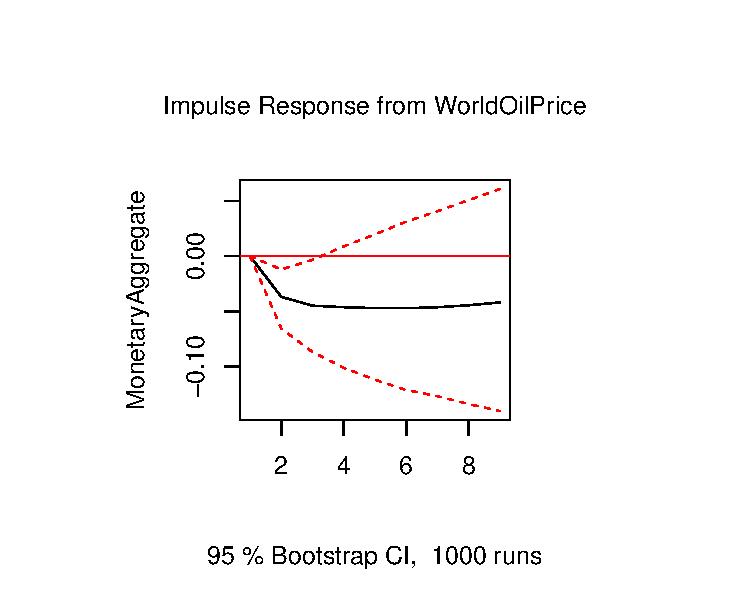
\includegraphics{README_files/figure-latex/unnamed-chunk-13-1} \end{center}

\begin{center}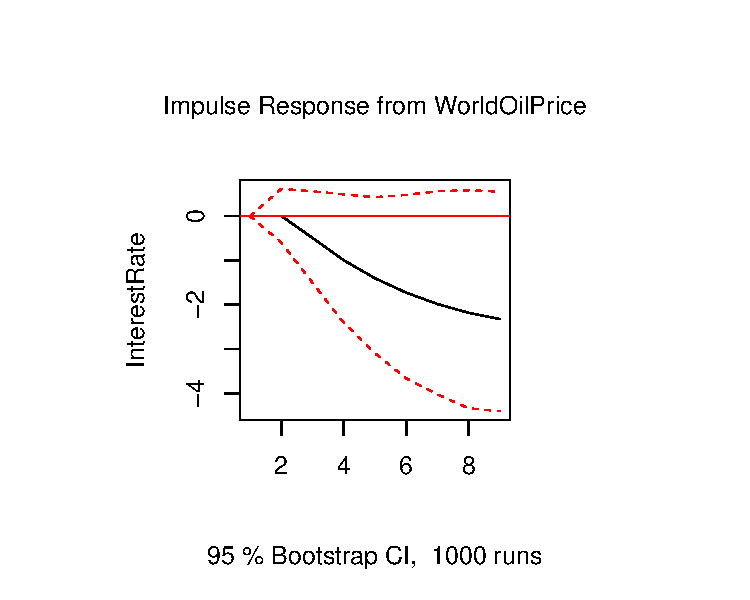
\includegraphics{README_files/figure-latex/unnamed-chunk-13-2} \end{center}

\begin{center}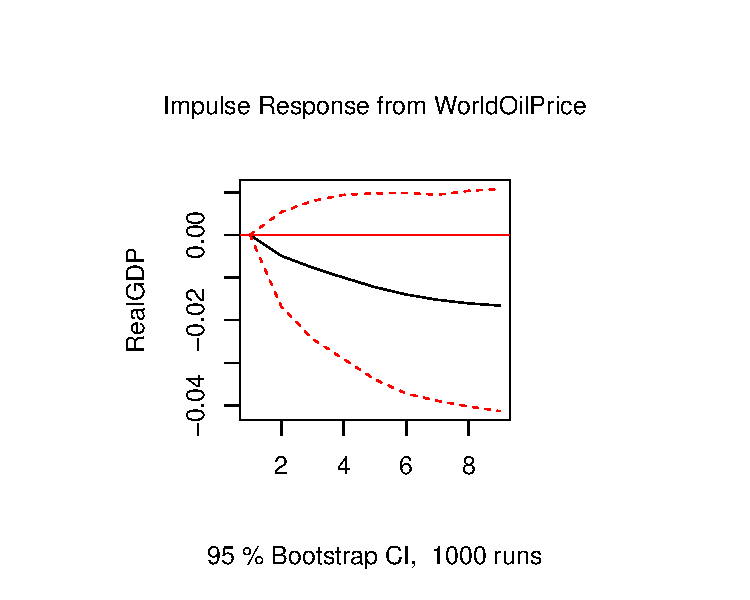
\includegraphics{README_files/figure-latex/unnamed-chunk-13-3} \end{center}

\begin{center}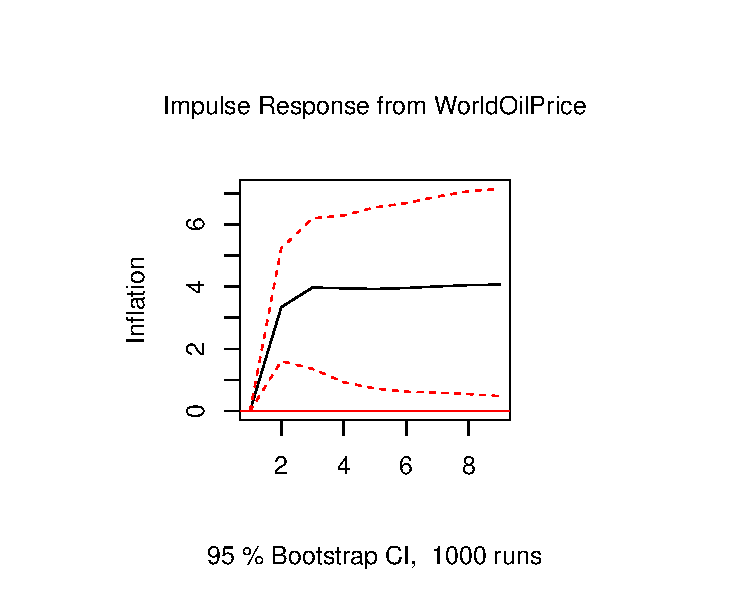
\includegraphics{README_files/figure-latex/unnamed-chunk-13-4} \end{center}

\begin{center}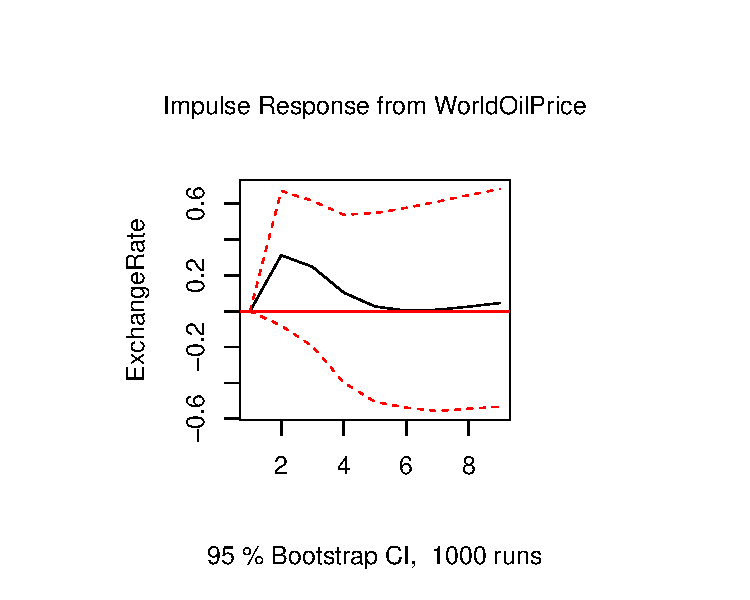
\includegraphics{README_files/figure-latex/unnamed-chunk-13-5} \end{center}

Cointegrating vectors visually??

\ldots Let us see if we can impose the restrictions contained in the B
matrix onto the cointegrating vectors contained in the Et matrix.

\begin{verbatim}
## #############
## ###Model VECM 
## #############
## Full sample size: 108    End sample size: 104
## Number of variables: 6   Number of estimated slope parameters 126
## AIC -3210.216    BIC -2855.868   SSR 74.89496
## Cointegrating vector (estimated by ML):
##    realGDP worldoilprice interestrate   inflation exchangerate
## r1       1             0   -0.1704922 -0.01710960    0.6161332
## r2       0             1    1.6056301  0.06991751   -5.4962156
##    monetaryaggregate
## r1        -0.3747751
## r2         6.5786487
## 
## 
##                            ECT1                ECT2               
## Equation realGDP           0.0114(0.0262)      0.0012(0.0029)     
## Equation worldoilprice     -1.1213(0.6892)     -0.1191(0.0757)    
## Equation interestrate      -0.8253(1.3364)     -0.0909(0.1468)    
## Equation inflation         1.9807(4.2269)      0.2323(0.4642)     
## Equation exchangerate      -1.5280(0.4970)**   -0.1498(0.0546)**  
## Equation monetaryaggregate -0.0999(0.0543).    -0.0127(0.0060)*   
##                            Intercept             realGDP -1          
## Equation realGDP           -0.2387(0.5689)       0.3017(0.1198)*     
## Equation worldoilprice     23.9522(14.9378)      6.0850(3.1445).     
## Equation interestrate      18.0500(28.9642)      9.3757(6.0972)      
## Equation inflation         -43.1723(91.6115)     23.9182(19.2849)    
## Equation exchangerate      31.3052(10.7722)**    0.0695(2.2676)      
## Equation monetaryaggregate 2.3668(1.1764)*       -0.2741(0.2476)     
##                            worldoilprice -1    interestrate -1    
## Equation realGDP           -0.0015(0.0061)     -0.0022(0.0021)    
## Equation worldoilprice     0.4921(0.1589)**    -0.0330(0.0553)    
## Equation interestrate      0.5017(0.3081)      0.5658(0.1072)***  
## Equation inflation         4.0209(0.9746)***   -0.8458(0.3391)*   
## Equation exchangerate      0.3216(0.1146)**    0.0338(0.0399)     
## Equation monetaryaggregate -0.0342(0.0125)**   0.0027(0.0044)     
##                            inflation -1        exchangerate -1    
## Equation realGDP           -0.0007(0.0010)     0.0030(0.0035)     
## Equation worldoilprice     -0.0649(0.0261)*    0.0232(0.0930)     
## Equation interestrate      -0.1333(0.0505)**   -0.0459(0.1802)    
## Equation inflation         -0.3031(0.1598).    0.2740(0.5701)     
## Equation exchangerate      -0.0376(0.0188)*    -0.2884(0.0670)*** 
## Equation monetaryaggregate 0.0093(0.0021)***   -0.0107(0.0073)    
##                            monetaryaggregate -1 realGDP -2           
## Equation realGDP           -0.0421(0.0628)      0.2444(0.1211)*      
## Equation worldoilprice     -0.5255(1.6486)      1.0297(3.1793)       
## Equation interestrate      -0.7766(3.1966)      -0.0562(6.1646)      
## Equation inflation         1.3461(10.1107)      -10.4541(19.4983)    
## Equation exchangerate      -0.3822(1.1889)      -5.2154(2.2927)*     
## Equation monetaryaggregate 0.3084(0.1298)*      -0.4686(0.2504).     
##                            worldoilprice -2    interestrate -2   
## Equation realGDP           0.0033(0.0061)      0.0020(0.0025)    
## Equation worldoilprice     0.0529(0.1609)      0.0008(0.0653)    
## Equation interestrate      -0.3103(0.3121)     0.0588(0.1266)    
## Equation inflation         0.8367(0.9870)      0.1164(0.4004)    
## Equation exchangerate      0.0028(0.1161)      0.0796(0.0471).   
## Equation monetaryaggregate -0.0030(0.0127)     0.0014(0.0051)    
##                            inflation -2        exchangerate -2    
## Equation realGDP           -0.0010(0.0010)     -0.0023(0.0034)    
## Equation worldoilprice     -0.0211(0.0266)     -0.0957(0.0890)    
## Equation interestrate      0.0222(0.0516)      -0.1919(0.1725)    
## Equation inflation         -0.1823(0.1633)     -0.6758(0.5456)    
## Equation exchangerate      -0.0071(0.0192)     -0.1283(0.0642)*   
## Equation monetaryaggregate 0.0023(0.0021)      -0.0097(0.0070)    
##                            monetaryaggregate -2 realGDP -3          
## Equation realGDP           0.0925(0.0628)       -0.0572(0.1260)     
## Equation worldoilprice     2.1871(1.6496)       -1.6558(3.3091)     
## Equation interestrate      4.6408(3.1985)       5.5340(6.4163)      
## Equation inflation         4.7544(10.1165)      -8.8125(20.2941)    
## Equation exchangerate      0.7138(1.1896)       -10.8377(2.3863)*** 
## Equation monetaryaggregate -0.0451(0.1299)      0.2839(0.2606)      
##                            worldoilprice -3   interestrate -3    
## Equation realGDP           0.0061(0.0059)     0.0007(0.0022)     
## Equation worldoilprice     0.2848(0.1541).    0.0895(0.0570)     
## Equation interestrate      1.2330(0.2988)***  0.0649(0.1105)     
## Equation inflation         0.4219(0.9450)     0.9330(0.3494)**   
## Equation exchangerate      0.3740(0.1111)**   -0.0451(0.0411)    
## Equation monetaryaggregate -0.0218(0.0121).   -0.0080(0.0045).   
##                            inflation -3        exchangerate -3    
## Equation realGDP           -0.0016(0.0010)     0.0017(0.0034)     
## Equation worldoilprice     -0.0329(0.0258)     -0.0271(0.0888)    
## Equation interestrate      -0.1358(0.0500)**   -0.0992(0.1721)    
## Equation inflation         -0.0726(0.1580)     -0.5133(0.5445)    
## Equation exchangerate      -0.1181(0.0186)***  -0.0048(0.0640)    
## Equation monetaryaggregate 0.0050(0.0020)*     -0.0079(0.0070)    
##                            monetaryaggregate -3
## Equation realGDP           -0.0568(0.0583)     
## Equation worldoilprice     -0.4480(1.5304)     
## Equation interestrate      1.7129(2.9674)      
## Equation inflation         -1.4109(9.3857)     
## Equation exchangerate      3.0424(1.1036)**    
## Equation monetaryaggregate 0.0729(0.1205)
\end{verbatim}

\#Find VECM residuals

We want to compare our estimates to the one in Table 3.

Maybe instead it is the VAR system \ldots missing constant and trend

Then test for white noise residuals.

\hypertarget{step-6-is-it-stationary}{%
\section{Step 6: Is it stationary?}\label{step-6-is-it-stationary}}

\hypertarget{step-7-are-the-residuals-white-noise}{%
\section{Step 7: Are the residuals white
noise?}\label{step-7-are-the-residuals-white-noise}}

\hypertarget{step-8-find-vecm-model-by-imposing-sr-contemporaneous-effects}{%
\section{Step 8: Find VECM model by imposing SR contemporaneous
effects}\label{step-8-find-vecm-model-by-imposing-sr-contemporaneous-effects}}

\hypertarget{step-9-test-model-specification-using-congruency-parsimony-lag-inclusion}{%
\section{Step 9: Test model specification using congruency, parsimony,
lag
inclusion\ldots{}}\label{step-9-test-model-specification-using-congruency-parsimony-lag-inclusion}}

Alternatively, exclude exchange rates as the paper unusually included
these. However, in our models we could not find exchange rates to be
significant.

\hypertarget{appendix}{%
\section*{Appendix}\label{appendix}}
\addcontentsline{toc}{section}{Appendix}

\hypertarget{johansen-tests}{%
\section*{Johansen Tests}\label{johansen-tests}}
\addcontentsline{toc}{section}{Johansen Tests}

\bibliography{Tex/ref}





\end{document}
